\documentclass[final]{article}

% if you need to pass options to natbib, use, e.g.:
% \PassOptionsToPackage{numbers, compress}{natbib}
% before loading nips_2017
%
% to avoid loading the natbib package, add option nonatbib:
% \usepackage[nonatbib]{nips_2017}

\usepackage{nips_2017}
\usepackage{graphicx,url}
\usepackage{amsmath}
\usepackage{amssymb}
\usepackage{balance}
\usepackage{gensymb}
\usepackage{multirow}
\usepackage{hhline}
\usepackage{array}
\usepackage[font=small,labelfont=bf]{caption}
\usepackage{dblfloatfix}
\usepackage{gensymb}
\usepackage{tabu}
\usepackage[dvipsnames]{xcolor}
% to compile a camera-ready version, add the [final] option, e.g.:
% \usepackage[final]{nips_2017}

\usepackage[utf8]{inputenc} % allow utf-8 input
\usepackage[T1]{fontenc}    % use 8-bit T1 fonts
\usepackage{hyperref}       % hyperlinks
\hypersetup{
    colorlinks=true,
    linkcolor=blue,
    filecolor=magenta,      
    urlcolor=blue,
}
\usepackage{url}            % simple URL typesetting
\usepackage{booktabs}       % professional-quality tables
\usepackage{amsfonts}       % blackboard math symbols
\usepackage{nicefrac}       % compact symbols for 1/2, etc.
\usepackage{microtype}      % microtypography
\newcommand{\code}[1]{\texttt{#1}}
\newcommand{\cmdline}[1]{\colorbox{gray!30}{\texttt{#1}}}

\title{Assignment 1: Localization with Particle Filters}

\begin{document}
%\nipsfinal

\maketitle

In this assignment you will implement a particle filter to localize your car within a known map. This will provide a global pose ($\mathbf{x_t} = <x_t, y_t, \theta_t>$) for your car where ($x_t$, $y_t$) is the 2D position of the car within the map and $\theta_t$ is the heading direction w.r.t. the map's frame of reference. You will be implementing different parts of the particle filter, namely the motion model, sensor model, and the overall filtering framework. You will also be tuning various parameters that govern the particle filter to gain intuition on the filter's behaviour. The provided skeleton code has enough to get you started, as well as data and code for testing different aspects of your particle filter. Make sure the assignment directory (lab\_1) is in \code{$\sim$/catkin\_ws/src} and to run \code{source $\sim$/.bashrc \&\& cd $\sim$/catkin\_ws \&\& catkin\_make}.

This assignment can be done as a group. Only one member of the group needs to submit the assignment. All group members' names should be on the document containing answers to the assignments' questions. Additionally, there will be a final demo where we will meet with each team to test their particle filter on actual runs through the basement in Allen building.

\section{Getting Started}

Here is some \textbf{very important} prerequisite information for this assignment:

\begin{itemize}
\item This assignment references sections of \textit{Probabilistic Robotics} by Sebastian Thrun, Wolfram Burgard, and Dieter Fox. It is an excellent book that if you are interested in pursuing robotics we recommend reading. But you can likely find a PDF version online for the purposes of this assignment.
\item In the past, this assignment has taken a lot of time for students to complete. We have since simplified it and made it easier to tune your particle filter. Regardless, start early on this assignment. In addition, make sure that both the motion model and sensor model match our expectations before testing the particle filter otherwise you will see poor results. 
\item Students have said tuning takes the most time. We set the tuning values roughly to what you want, but you will still need to tune. The key to tuning is first understanding what you are tuning, \textit{Probabilistic Robotics} can help with that. Then tune one thing at a time, gradually.
\item Computation should be done \textit{in-place}, particularly when updating \code{self.particles} and/or \code{self.weights}. For example, updating the \code{self.weights} \textit{in-place} means that the result of the update should be stored in the \code{self.weights} array, rather than returning a new array that contains the result of the update. Note that, at least in this context, doing an in-place update does not mean that you cannot use intermediate arrays and/or data structures to perform the calculation. It only specifies that the values of an array (such as \code{self.particles} or \code{self.weights}) should be updated with the result of the computation, rather than returning a whole new array.

\item Emphasizing the point above, when updating the values of \code{self.particles} and/or \code{self.weights}, make sure that you are updating the \textit{values} of the array, rather than changing the array that \code{self.particles} and/or \code{self.weights} refers to. Different modules each contain their own references to \code{self.particles}, but they all refer to the same array (the same can be said for \code{self.weights}). Therefore changing the array that \code{self.particles} and/or \code{self.weights} references in one module will cause the other modules to no longer see the updates made by that module (and vice-versa). For example, doing something of the form \code{self.weights = a} would be very bad; instead one could use \code{self.weights[:] = a[:]} to update the \code{self.weights} array.

\item The particle filter algorithm that we wrote in class contains a number of for-loops. However, for most of these for-loops, the iterations are independent of each other. Therefore we can turn many of these for-loops into vector computations. For example, instead of sampling particles one at a time from the motion model, you can receive a whole vector of sampled particles. You should do vectorized computations whenever possible in order to write efficient code - failing to do so could cause your particle filter to not run sufficiently fast.

\item We gave you some useful utility functions in utils.py. Check it out!

\end{itemize}

\section{ Motion Model}
As discussed in class, a motion model specifies the probability distribution $p(\mathbf{x}_t | \mathbf{x}_{t-1}, u_t)$, i.e. the probability of reaching a pose $\mathbf{x}_t$ given that we apply a control $u_t$ from pose $\mathbf{x}_{t-1}$. Unlike a traditional Bayes filter which requires us to explicitly represent the posterior over possible future poses (i.e. explicitly compute $p(\mathbf{x}_t | \mathbf{x}_{t-1}, u_t)$),  we only need to be able to draw samples from this distribution for the particle filter:
\begin{equation}
\mathbf{x}^\prime_t \sim p(\mathbf{x}_t | \mathbf{x}_{t-1}, u_t) 
\end{equation}
where $\mathbf{x}^\prime_t$ is a possible next pose ($x_t,y_t,\theta_t$) sampled from the motion model. We will be using the kinematic car model for this assignment. See the Kinematic\_Car\_Model.pdf for the derivation.

\textbf{Question: What assumptions is this model making? (list a few)}

\subsection{Noise}
The kinematic car model makes deterministic predictions, i.e. given an initial pose $\mathbf{x}_{t-1}$ and control $u_t$ there is a single predicted future pose $\mathbf{x}_t$. This would be acceptable if our model is perfect, but as you have seen we have made many simplistic assumptions to derive this model. In general, it is very hard to model any physical process perfectly. In practice, we would like our model to be robust to  potential errors in modeling. We do this by allowing our model to be probabilistic - given any pose $\mathbf{x}_{t-1}$ and control $u_t$, our model can predict a distribution over future states $\mathbf{x}_t$, some being more likely than others. We achieve this by sampling noisy controls from the nominal controls $\bar{v_t}$ and $\bar{\delta_t}$, propogating those controls through the kinematic car equations to get prediction $\bar{x_t} = f[x_{t-1},u_t]$, and finally adding model noise to the output. Mathematically: 

\begin{align*}
u_t =& <v_t, \delta_t>, v_t \thicksim N(\bar{v_t},\sigma_v), \delta_t \thicksim N(\bar{\delta_t}, \sigma_{\delta}) \\
\bar{x_t} =& f[x_{t-1},u_t] \\
x_t \thicksim & N(\bar{x_t}, \sigma_{x_t})
\end{align*}
It will be up to you to pick reasonable noise parameters that determine the widths of the various gaussians that must be sampled from.

\begin{figure*}[!htb]
\centering
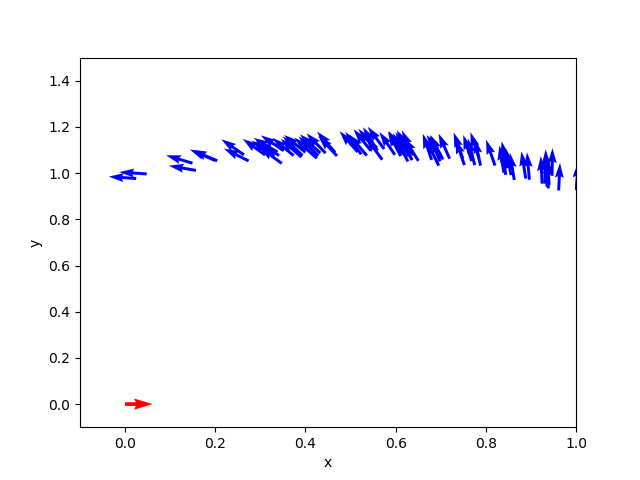
\includegraphics[width=0.5\linewidth]{figs/motion_model.png}
\caption{Propagation of particles when moving forward and to the left. The banana curve is expected when noise is added to the system. Red is the expected start pose, Blue is the particles after the control}
\label{fig:motion_model}
\end{figure*}
\subsection{Motion Model Implementation}
Implement the motion model in the provided \textbf{MotionModel.py} script found the \code{/src} directory. Make sure to only fill in the functions that say YOUR CODE HERE according to the function description, inputs, and required outputs.

All tuning parameters are provided at the top of \textbf{MotionModel.py} with their descriptions. The initial values are ballparks of what you should set.

Test your motion model by running the \textbf{TestMM.py} script. Make sure your motion model passes all tests. DO NOT EDIT \textbf{TestMM.py}. If some tests are failing and you are getting a banana curve, look at \textbf{TestMM.py} to help determine the test you are failing. You should also see a visualization similar to Figure \ref{fig:motion_model}.

\textbf{Question: Why are so many particles in a 10cm radius of the ground truth for test 1 as opposed to test 2/3?}


\section{Sensor Model}

The sensor model captures the probability $p(\mathbf{z}_t | \mathbf{x}_t,\mathbf{m})$ that a certain observation $\mathbf{z}_t$ can be obtained from a given robot pose $\mathbf{x}_t$ (assuming that the map of the environment is known). In this assignment, $\mathbf{z}_t$ is the LIDAR data from the laser sensor mounted on the robot. Your task in this section is to implement and analyze the LIDAR sensor model discussed in class.

The LIDAR sensor shoots out rays into the environment at fixed angular intervals and returns the measured distance along these rays (or NAN and/or 0.0 for an unsuccesful measurement). Therefore, a single LIDAR scan $\mathbf{z}$ is a vector of distances along these different rays $\mathbf{z} = \left[z^1, z^2, ...., z^N\right]$. Given the map of the environment ($m$), these rays are conditionally independent of each other, so we can rewrite the sensor model likelihood as follows:
\begin{align}
p(\mathbf{z}_t | \mathbf{x}_t, m) = p(z_t^1, z_t^2, ...., z_t^N | \mathbf{x}_t, m) = p(z_t^1 | \mathbf{x}_t, m) * p(z_t^2 | \mathbf{x}_t, m) * ... * p(z_t^N | \mathbf{x}_t ,m )
\end{align}
where the map $m$ is fixed (we will not use $m$ explicitly in any further equations, it is assumed to be provided). As we can see, to evaluate the likelihood it is sufficient if we have a model for measuring the probability $p(z_t^k | \mathbf{x}_t)$ of a single range measurement given a pose.\newline
\break
\textbf{Question: What are the drawbacks of viewing each ray as conditionally independent?}

We will compute this in the following manner: First, we will generate a simulated observation $\hat{\mathbf{z}}_t$ given that the robot is at a certain pose $\mathbf{x}_t$ in the map. We do this by casting rays into the map from the robot's pose and measuring the distance to any obstacle/wall the ray encounters. This is very much akin to how laser light is emitted from the LIDAR itself. We then quantify how close each ray in this simulated observation $\mathbf{z}_t^{k^*}$ is to the real observed data $\mathbf{z}^k_t$, which provides an estimate of $p(z_t^k | \mathbf{x}_t)$. 

Overall, this requires two things: 
\begin{enumerate}
\item A way to compute the simulated observation given a pose
\item A model that measures closeness between the simulated and real data
\end{enumerate}

For the purpose of this assignment, we will use a raycasting library called rangelibc (implemented in C++/CUDA) to compute the simulated observation. The second part is what you will be implementing - a model that measures how likely you are to see a real observation $\mathbf{z}^k_t$ given that you are expected to see a simulated observation $\mathbf{z}_t^{k^*}$. The LIDAR sensor model we use is a combination of the four curves shown in Figure 6.3 \textit{Probabilistic Robotics} with the exception of \(P_{short}\) which we will model as linear. 
\[
P_{short}(z_t^k | x_t) = \left\{
\begin{array}{@{}ll@{}}
2\frac{z_t^{k^*} - z_t^k}{z_t^{k^*}}, & z_t^k < z_t^{k^*}\\
0, &\text{otherwise}
\end{array}\right.
\]
Certain mixing parameters and hyper-parameters that weight each of the four components against the other will be chosen by you. To understand this model and how to combine these curves look at Section 6.3.1 of \textit{Probabilistic Robotics}. There is a good description in there about the high level ideas and the implementation. Note, this is only one way of many ways to compute $p(\mathbf{z}_t | \mathbf{x}_t,\mathbf{m})$.

Given that the LIDAR range values are discrete (continuous values are converted to discrete pixel distances on the 2D map), we do not have to generate the model on-line and can instead pre-calculate them. This will be represented as a table of values, where each row is the actual measured value and the column is the expected value for a given LIDAR range. Pre-computing this table allows for faster processing during runtime. During run-time, we use the aforementioned ray casting library to generate simulated range measurements. We then look-up in the table the simulated (column) and real measurements (row) and get a probability.

\textbf{Question: What assumptions is this model making? (list a few)}
\subsection{Noise}
Noise in the sensor model is based on the gaussian defining \(P_{hit}\). With high noise (high variance), the probability of a accurate measurement is lower. Checkout equation 6.5 in section 6.3 of \textit{Probabilistic Robotics} for more insight. Don't worry about the normalizer mentioned there, we will normalize at the end.

\[
P_{hit}=\left\{
\begin{array}{@{}ll@{}}
\mathcal{N}(z_t^k;z_t^{k^*},\sigma_{hit}^2), & 0 \leq z_t^k \leq z_{max}\\
0, &\text{otherwise}
\end{array}\right.
\]

\subsection{Sensor Model Implementation}
For this part of the assignment, you will implement the sensor model in the file \textbf{SensorModel.py}. In particular, the function \code{precompute\_sensor\_model()} should return a \code{numpy} array containing a tabular representation of the sensor model. The code provided will use your array as a look-up table to quickly compare new sensor values to expected sensor values, returning the final sensor model likelihood: $p(\mathbf{z}_t | \mathbf{x}_t)$.

All tuning parameters are provided at the top of \textbf{SensorModel.py} with their descriptions. The initial values are ballparks of what you should set.

Test your sensor model by running the \textbf{TestSM.py} script. DO NOT EDIT \textbf{TestSM.py}. It will return heatmaps illustrating which locations are most likely. The expected outputted heatmaps can be found in \code{/plots}. Note that your results will differ depending on the sensor model parameters that you choose but you should try to match the heatmaps as close as possible. We are looking for something similar to the plots, not exactly the same. Pay attention to the locations of the small white dots in the heatmap, that is what we will be looking for.

\textbf{Question: Why does the hallway heatmap not converge on one point?}

\section{Particle Filter}
 In the particle filter, your belief over the robot pose $Bel(\mathbf{x}_t)$ is represented as a list of $M$ particles (these are nothing but samples from the belief distribution). Each particle $i$ has a pose $\mathbf{x}^i_t$ which represents a hypothetical robot at that particular pose; using many particles allows for us to more accurately represent the belief distribution. The trade-off is with more particles you may be more accurate but at the cost of added computation. Further description of the particle filter algorithm can be found in section 4.3.1 of \textit{Probabilistic Robotics}. 

Note that, in this assignment the particles and weights are updated asynchronously. Specifically, the motion model is applied whenever messages about the speed of the motor and steering angle are received. The sensor model is applied whenever a laser scan is received, which also triggers the weighted re-sampling of particles shortly after. This asynchronous structure allows us to utilize all of the messages that are received, rather than operating at the rate of the slowest topic.

From a high level, this is how the particle filter works. Initially, we have a prior belief over where the robot is: $Bel(\mathbf{x}_0)$. RVIZ enables you to specify the initial pose of the robot - this will specify $Bel(\mathbf{x}_0)$. We will represent this belief using a fixed number of $M$ particles - initially all these particles will be gaussian distributed around the clicked pose. In order to specify a pose, look for a button labeled \textbf{2D Pose Estimate} along the top bar of the RVIZ interface. After clicking this button, you  can specify a position and orientation by clicking and dragging on the map. Next, each particle will be propagated forward in time using the motion model whenever you move the car. Using ray-casting, we will generate a simulated LIDAR observation for each particle which we will compare to the real LIDAR data from the laser sensor. This now assigns a ``weight'' for each particle - particles with higher weights are more likely given the motion and sensor model updates. Finally, we will re-sample from this distribution to update our belief over the robot's pose $Bel(x_t)$ - this resampling step gets rid of particles with low belief and concentrates our distribution over particles with higher belief. We repeat these steps recursively.

\subsection{Particle Filter Implementation}
In this part of the assignment, you will be implementing a particle filter to track our belief over the robot's pose over time with a fixed number of particles. The code from the prior sections will be used in the file \textbf{ParticleFilter.py}. You will implement functions in \textbf{ParticleFilter.py} to initialize the belief of the robot. See the skeleton code for more details. Make sure to only fill in the functions that say YOUR CODE HERE according to the function description, inputs, and required outputs.

In prior sections, you implemented algorithms for sampling from a motion model with noise and evaluating a sensor model. The key step remaining is to implement the re-sampling step (discussed in the next section).

\subsection{Low Variance Re-sampling}
You will implement a low-variance re-sampler for your particle filter in \textbf{ReSample.py}. Instead of re-sampling randomly with a higher probability for higher weighted items, we will do a sequential re-sampling. The ideas is to line up a series of intervals associated with each particle. Each interval's size is equivalent to the normalized weight. If we are trying to draw \(M\) samples, we will choose a random number \(r\in [0,M^{-1}]\). We then draw samples by checking which interval \(r\) is in and updating \(r\) by \(r = r + M^{-1}\). A full description of the algorithm can be found in Table 4.4 of \textit{Probabilistic Robotics}. Figure \ref{fig:resample} from \textit{Probabilistic Robotics} shows this visually.

There are three advantages of the low-variance re-sampler. One, it will sample more evenly over all particles, instead of the possibility of sampling only small subregion of the particles. Two, if all weights are the same, it will sample all of them, so no samples are lost. Three, its complexity is \(O(M)\) as opposed to the random sampler \(O(MlogM)\) which will be important for real time performance.

\begin{figure}
    \centering
    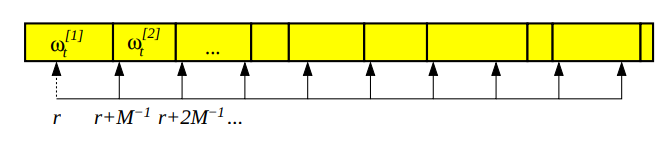
\includegraphics[width=0.8\linewidth]{figs/resample.png}
    \caption{Principle of the low variance resampling procedure. We choose a random number \(r\) and then select those particles that correspond to \(u = r + (m - 1) \cdot M^{-1}\) where \(m = 1, . . . , M\)}
    \label{fig:resample}
\end{figure}

\subsection{Re-Sampler Visualization}
Implement a low-variance re-sampler for your particle filter in \textbf{ReSample.py}. We will visualize the samples that our re-sampler methods are drawing. To test the sampler we will repeatedly sample from a particle distribution where the weights are defined as follows:

\[
	w_i = 
	\begin{cases}
	\frac{i}{\Sigma w_i} & \text{if } i < k\\
	0 & \text{if } i >= k
	\end{cases}
\]

Where $k$ is some value less than the the number of weights. To test your code run \textbf{TestRS.py}. \textbf{TestRS.py} samples from this particle distribution \textit{trials} number of times, and then creates a histogram of how many times each particle was sampled across all trials. DO NOT EDIT \textbf{TestRS.py}. You should see plots similar to the ones found in \code{/plots} for the various values of \(k\).

\textbf{Question: Why do the samples close to k get sampled more?}

\subsection{Testing Particle Filter in Simulation with Teleoperation}
\label{sec:test_pf_sim_teleop}
You can test your particle filter in simulation by doing the following:

\begin{enumerate}
\item Change the map arg in \code{$\sim$/catkin\_ws/src/mushr\_sim/launch/map\_server.launch} to \code{cse\_022} from package \code{lab\_1} as you did in \code{lab\_0}.
\item Run \code{roscore}
\item Launch the test file: \cmdline{roslaunch lab1 TestPF\_sim.launch}
\item Open rviz, \cmdline{rviz}, and visualize the following topics:
\begin{itemize}
    \item \code{/map} Map topic
    \item \code{/pf/particles} PoseArray topic
    \item \code{/pf/inferred\_pose} Inferred Pose topic
    \item \code{/scan} LaserScan topic
    \item \code{/car\_pose} ground truth Pose
\end{itemize}
\item Wait for the terminal to output \code{Vesc callback called for first time....} then click the \textbf{2D Pose Estimate} button, and click and drag on the map to set a start pose. All of the particles should then redistribute around this pose.
\item Teleoperate the car. The particle filter's estimate of the robot's state should approximately correspond to the true pose of the robot in the map.
\end{enumerate}
After you are satisfied with your particle filter's performance, change the \code{"plot"} argument to "true" in \code{TestPF\_sim.launch}. Then rerun the above steps, after some time a plot showing the true and pf trajectory should come up. \textbf{Submit this plot}. Do not drive the car backwards as it makes for messy plots. If you want to test your particle filter in sim without it relaunch the sim each time run \code{ParticleFilter\_Sim.launch}


\subsection{Testing Particle Filter with a Bag File}
\label{sec:test-pf-bag}
We have provided a number of bags for testing your particle filter implementation under the \code{bags/testing/} directory. These bags contain all of the data necessary to run the particle filter, as well as the output of our particle filter when processing the data. 
To test the particle filter, do the following:
\begin{enumerate}
\item Change the \code{bagfile} parameter of \code{TestPF\_bag.launch} to one of the maps in \code{/bags/testing/}
\item run \code{roscore}
\item Launch rviz. This is an important step as the map is only published at the beginning so make sure to run rviz before launching test code.
\item Launch the test file: \cmdline{roslaunch lab\_1 TestPF\_bag.launch}
\item Visualize following topics:
	\begin{itemize}
	    \item The \code{/map} Map topic
		\item The \code{/pf/inferred\_pose} Pose topic
		\item The \code{/scan} LaserScan topic
		\item The \code{/pf/ta/viz/inferred\_pose} Pose topic
	\end{itemize}
\end{enumerate} 

The output of our particle filter implementation is published to topics that are prefixed with \code{/pf/ta/viz}, while the outputs of your implementation will publish to topics prefixed with \code{/pf/}. If you view these topic in rviz, you can compare the performance of your particle filter to our implementation. Though it is unlikely that both filters will produce exactly the same results, the expected poses of both filters should be similar at all times. The terminal will print the median \(x,y,\theta\) errors. At the end of the run on \code{full.bag} your \textbf{median errors should all be less than 0.01}.

\subsection{Testing Particle Filter on Robot}

Run your particle filter code directly on the robot, and \textbf{record the bag file}. To do this, you should use the scp command to copy your \code{lab\_1} directory directly into the \code{catkin\_ws/src} directory on the robot. Then run \code{catkin\_make} in the robot's \code{catkin\_ws} directory.

\begin{enumerate}
\item Change the \code{map} parameter in \code{mushr\_base} to find \code{cse022.yaml} in  \code{lab\_1/maps/}. To find \code{map\_server.launch}: \cmdline{roscd mushr\_base/launch/includes}
\item Launch teleop.launch: \cmdline{roslaunch mushr\_base teleop.launch}
\item Launch map\_server.launch: \cmdline{roslaunch mushr\_base map\_server.launch}
\item Launch ParticleFilter.launch: \cmdline{roslaunch lab\_1 ParticleFilter.launch}
\item Make sure that your ROS\_IP and ROS\_MASTER\_URI are set correctly. IP should be set on the car and computer to their appropriate IP addresses and URI should be set to the car IP. See \href{http://wiki.ros.org/ROS/EnvironmentVariables#ROS_MASTER_URI}{here} for more info.
\item Open rviz and visualize:
	\begin{itemize}
	    \item The \code{/map} Map topic
		\item The \code{/pf/inferred\_pose} Pose topic
		\item The \code{/scan} LaserScan topic
		\item The \code{/pf/particles} PoseArray topic
	\end{itemize}
\item Click the \textbf{2D Pose Estimate} button, and click and drag on the map according to where the robot actually is in the map. All of the particles should then redistribute around this pose.
\item Teleoperate the car. The particle filter's estimate of the robot's state should approximately correspond to the true pose of the robot in the map.
\end{enumerate}

Steps 4 through 7 should be done on your own computer. Note that now when you specify the initial pose in rviz, it should correspond to where the robot really is, not some arbitrary starting point in the map. Record a bagfile of your car driving around the localization corner. We will not accept large bag files (200 mb+). To make the bag files small, do not record the image topics. See \href{http://wiki.ros.org/rosbag/Commandline#record}{rosbag record} for more details.

\textbf{Question: Where does the particle filter do well? Where does it fail? Why?
Hint: It shouldn't work perfectly all the time.}

\section{Extra Credit}

\subsection{Theory question}
Look at \code{/docs/Kinematic\_Car\_Model.pdf}. The model derived in the document is for the \emph{rear-axle}. 

\begin{enumerate}
	\item Derive the car model for the center of mass. 
	\item Derive the car model for the front axle.
\end{enumerate}

Your submission should include definitions for the following: \(\dot{x},\dot{y},\dot{\theta},x_{t+1}, y_{t+1},\theta_{t+1}\)

\subsection{Global localization}

Implement global localization at the start of the particle filter. So far, you’ve assumed access to a clicking interface which lets you manually initialize the robot’s pose. By implementing an algorithm for global localization, you can automate this process. There are multiple ways to do this: a naive way would be to increase the number of particles significantly until you are able to localize well globally right at the start. A better way would be to first initialize a large number of particles, weight these particles by the sensor model and sample a fixed number of $M$ particles from this weighted distribution. Can you come up with better ways to solve this problem? For this extra credit question, you will have to implement an algorithm that reliably localizes the robot at the start of the particle filter run without having to explicitly providing an initialization via clicking. Note that it does not have to lock on to the exact location right at the start as long as it is able to refine it’s belief estimate and converge to the correct distribution as the robot moves. 

Your submission should include code for global localization. You are free to edit the code however you like for this part. The TA’s will test this by having you re-initialize your particle filter in a new location without human input.

\subsection{Kidnapped robot}
Solve the kidnapped robot problem. A harder version of the global localization problem is called the kidnapped robot problem - say that your robot has been tracking the pose quite well, but suddenly a malicious agent picks the robot up while covering the LIDAR and moves it to a different location within the same map. Can your particle filter recover and correctly re-estimate this new position that the robot is in? Unlike the initial global localization problem, you now have an additional problem to solve - you have to figure out if you have been kidnapped and need to re-initialize your filter. 

Your submission should include code for re-initialization. You are free to edit the code however you like for this part. The TAs will test this by moving your robot to a new location in the middle of tracking while covering the LIDAR.

\section{Deliverables}
Submit all of your code and launch files. Your answers to questions should be in a file \code{writeup.txt}. All plots, bags, videos, and the writeup should be in the \code{/submission} directory. Tar your \code{lab\_0} package when you are done.

\subsection{Motion Model}
\begin{enumerate}
\item Run \textbf{TestMM.py}. Submit the figure it produces (in \code{/submission})
\item Question: What assumptions is this model making? (list a few)
\item Question: Why are so many particles in a 10cm radius of the ground truth for test 1 as opposed to test 2/3?
\end{enumerate}

\subsection{Sensor Model}
\begin{enumerate}
\item Run the code that visualizes your sensor model on each of the two provided laser scan bags. Submit the visualizations for both runs (in \code{/submission}).
\item Question: What are the drawbacks of viewing each ray as conditionally independent?
\item Question: What assumptions is this model making? (list a few)
\item Question: Why does the hallway heatmap not converge on one point?
\end{enumerate}

\subsection{Re-Sampler}
\begin{enumerate}
\item Run the code that visualizes the re-sampler. Submit all three visualizations (in \code{/submission}).
\item Question: Why do the samples close to k get sampled more?
\end{enumerate}

\subsection{Particle Filter}
\begin{enumerate}
\item Simulation: Submit the auto generated plot of your pf's trajectory with the true sim trajectory, as you drive the car around in sim. Hint: do not reverse, it makes for messy plots.
\item Bags: Submit the final median errors of your pf for all 3 files in \code{real\_floor4/}. Along with videos of each run in rviz. \textbf{Make sure to visualize all of the topics mentioned in Section \ref{sec:test-pf-bag}.} Show your particle filter's estimate of the expected pose in blue, and our recorded estimate in green.
\item Real Car: Submit the bag of your car running in one of the real world maps. \textbf{Make sure it is less than 200mb}. You should just drive the car around for a bit.
\item Question: Where does the particle filter do well? Where does it fail? Why? Hint: It shouldn’t work perfectly all the time.
\end{enumerate}

\section{Demo}

In your team’s demo to the TA’s, you will need to:
\begin{enumerate}
	\item Show the particle filter working on the robot car. The TAs will then drive your car around, and your particle filter should track the real world location reasonably.
of the car.
\end{enumerate}

\end{document}
